\section{Topology Optimization}
\label{sec:ToPy}
Due to the good range of topology optimization software available, we decided to adapt an open-source topology optimizer to our needs, namely \emph{ToPy}.


ToPy \cite{ToPy} is a python library/program, written by William Hunter and documented in \cite{Hunter2009}, implementing the SIMP model and method described in \autoref{subsec:TopOpTheory}. It is based on the 99-line Matlab code by Sigmund's for minimum compliance \cite{sigmund200199}. The program can optimize the previously named problem types: minimum compliance, heat conduction and mechanism synthesis --- in 2D as well as 3D. It uses highly optimized open source python libraries such as Pysparse \cite{Pysparse} and Numpy \cite{Numpy}, leading to improved speed, porta- and scalability. %The whole program is steered by an input file which-- with the help of the documentation-- is straightforward to use and easy to adapt. %citation on pysparse and numpy


%In terms of our implementation, 
We use ToPy as a black-box topology optimizer. This means, we launch the program with an input file based on our scenario and let ToPy run. Next, as soon as the output is available, we proceed with the next step. The intention is to create separate modules to be able to plug in different solvers later on. In order to specify our input, we wrote an auxiliary program taking a voxelized CAD design provided by CVMLCPP as input, outputting a .tpd file with geometry, load and fixture information in the format required by ToPy. 

Results of the topology optimization process can be seen in figure \ref{fig: topyStar}. Here, a star was given as input from a STL-file. We set the voxels in the star's points as fixtures, while we set a load in the middle, in the direction normal to the plane of the star. As can be seen, the optimization process "cuts" away unnecessary material in-between the corners and even in the middle of the material, returning an optimally stiff structure for the chosen remaining volume fraction. 
\begin{figure}
\centering
\begin{subfigure}{
  
\includegraphics[width=.2\linewidth]{Pictures/TopOp/Star_Optimized0_Trans.png}}
\end{subfigure}%
\begin{subfigure}{
  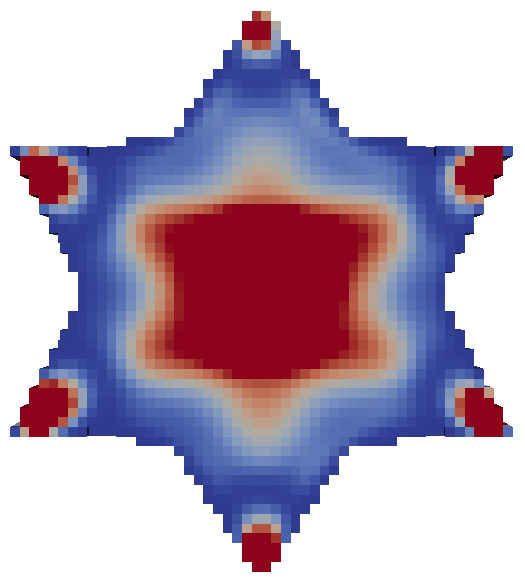
\includegraphics[width=.2\linewidth]{Pictures/TopOp/Star_Optimized2_Trans.png}}
\end{subfigure}
\begin{subfigure}{
  
\includegraphics[width=.2\linewidth]{Pictures/TopOp/Star_Optimized4_Trans.png}}
\end{subfigure}
\begin{subfigure}{
  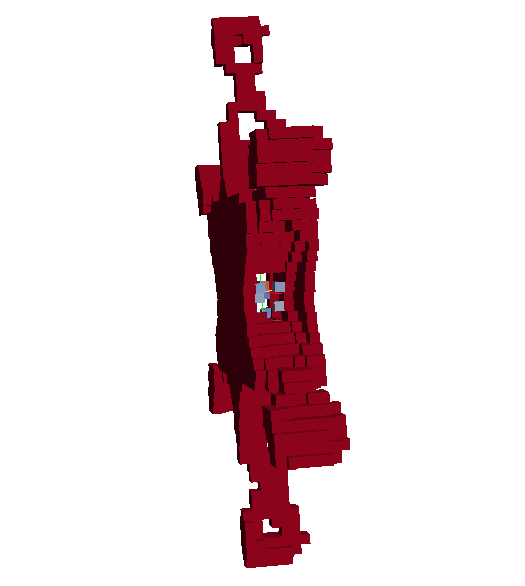
\includegraphics[width=.2\linewidth]{Pictures/TopOp/Star_Optimized5_Trans.png}}
\end{subfigure}
\caption{Topology Optimization by ToPy \cite{ToPy}, with minimum compliance. \emph{From left to right}: increasing number of SIMP iterations until convergence. The star-shaped structure was given by an STL-file which was processed into input readable by ToPy, with fixtures in the corners, and a load in the middle. Throughout the SIMP iterations, one can see how material from the less dense regions (blue) is concentrated into denser regions (red) that carry the load. The last picture gives a rotated view, to illustrate how material has been eliminated even from the inside of the star. } %which volume fraction?
\label{fig: topyStar}
\end{figure}
